% \section{Consistency Probing of Knowledge}
\section{Probing PLMs for Consistency}
\label{sec:probe}

In this section, we formally define consistency and describe
our framework for probing the consistency of PLMs.

\subsection{Consistency}
We define a model as \emph{consistent} if, given  two
\textit{cloze-phrases} such as 
 ``Seinfeld originally aired on [MASK]'' and
``Seinfeld premiered on [MASK]'' that
are \textit{quasi-paraphrases} it makes the same
prediction.\footnote{A \textit{quasi-paraphrase} --
  introduced by \citet{what_is_paraphrase} -- is a more
  fuzzy version of a paraphrase. The concept does not rely
  on the strict, logical definition of paraphrase and
  allows to operationalize concrete uses of
  paraphrases. This definition is in the spirit of the RTE
  definition \cite{dagan-rte}, which similarly supports a
  more flexible use of the notion of entailment.}
% \enote{hs}{I don't understand what this sentence says
% -- in  addition to what was previously already said:
  
% In the context of PLM knowledge consistency, if two cloze-phrases 
% % \yg{we didn't define cloze-phrases yet. do they include a relation tuple?} 
% of some relation (e.g., \textit{originally-aired-on}) are quasi-paraphrases, masked language models should predict the same entity for the masked item. 
% % \sr{I changed the wording here. Is it still what you meant? a natural question now is ``why objects".}
% % \yg{can it be "masked item"? or is it really a syntactic
% % object?}
% }
In the rest of the paper, we use the terms \textit{paraphrase} and \textit{quasi-paraphrase} interchangeably.

 
\enote{hs}{following paragraph: this sounds like quite a big
  problem to me: isn't it a huge assumption that the order
  of prediction will be the same for all paraphrases? is
  this seomthing we woudl expect of human performance?

  Can we move this to a later point in the paper and say:
  this is something that we will investigate in the future?}
We note that this definition does not take into account the type (e.g., one-to-one or many-to-many) of the relation. %\yg{what relation? we didn't say relation in this secction until now.} 
For instance, some relations are defined as \textit{many-to-many}, and as such, more than a single item can be factually correct, even for quasi-paraphrases. However, we still expect that the order will remain, and thus even if the alternative answer is factually correct, we still consider cases with different answers as a non-consistent result.
% \ar{Maybe we should report one-one and many-one separately, so that the reader can see both consistency and determinism results.}

\subsection{The Framework}
\label{sec:framework}

\begin{figure}[t!]
\centering

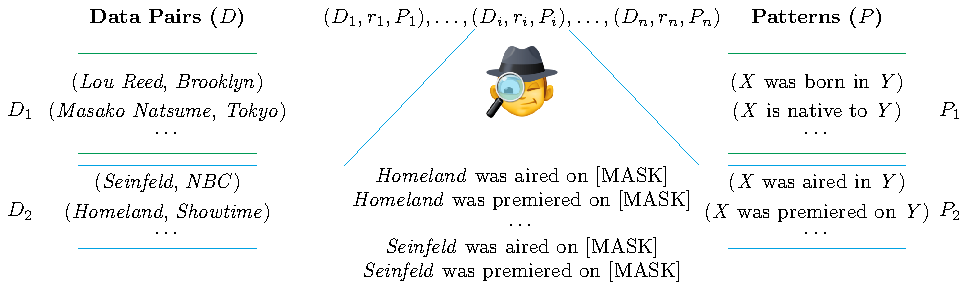
\includegraphics[width=1.\columnwidth]{figures/framework}

\caption{Overview of our framework that is used to assess models consistency.}
\label{fig:framework}
% \vspace{-6mm}
\end{figure}



\paragraph{New Trial}

An illustration of the framework is presented in Figure \ref{fig:framework}.
Let $D_i$ be a set of KB tuples of factual statements (e.g. <\textit{Homeland}, \textit{Showtime}>) from some relation $r_i$ (e.g. \textit{originally-aired-on}), accompanied with a set of \textit{quasi-paraphrases} cloze-patterns $P_i$ (e.g. \textit{X was originally aired on Y}).
Our goal is to test whether the model consistently predicts the same object (e.g. \textit{Showtime}) for a particular subject (e.g. \textit{Homeland}). To this end, we substitute X with a selected subject and Y with MASK (e.g. \textit{Homeland was originally aired on [MASK]}).
A consistent model must predict the same entity. Note that the consistency measure does not require the answers to be factually correct. While correctness is also an important property for KBs, we view it as a separate objective and measure it independently.


\paragraph{Previous Description}
Let $D = \{D_1, D_2, \dots, D_m\}$ be a set of sets of KB tuples, where each $D_i$ contains factual statements that express a specific relation $R_i$. In this section, we use $R_1$ = ``premiered on'' and $D_1$ as running examples. Each $D_i=\{d_1^i, d_2^i, \dots, d_n^i\}$ is composed of $n$ examples  where each $d_j^i = <s_j^i,o_j^i>$ is a subject-object tuple from the relation $R_i$. For example, $<\text{\textit{Homeland}}, \text{\textit{Showtime}}>$ is an example of a tuple in $D_1$. Each relation $R_i$ is associated with a set of cloze-patterns $P_i$ that are \textit{quasi-paraphrases} of each other, i.e., they express the same relation $R_i$. For example, $P_1=\{p_1^1, p_2^1, \dots, p_n^1\}$ contains the patterns ``\subj{} was originally aired on \obj{}'' and ``\subj{} premiered on \obj{}''. \nk{I think we should have someone who is not familiar with our setup check this passage. I am not sure if everyone will understand it}
\yg{I agree, hard to follow. I propose to possible solutions: (1) start bottom-up rather than top-down: this is a pattern, here is a group of patterns, now we collect them into a set... (2) visualize it in a figure (instead of the text).}
\am{while I'm familiar with this work, reading this paragraph for the first time I can understand the definitions. I agree with Yoav that a visualization can help though}
\enote{hs}{I do think the reader has to put in a little bit   of effort, but I'm the type of writer who expects that of   the reader. I agree that we should consider a figure!}

Given some relation $R_i$, a subject-object tuple $d_j^i \in D_i$ (e.g., `Homeland', `Showtime') and two paraphrases $p_k^i, p_l^i \in P_i$ associated with this relation (such as ``\subj{} was originally aired on \obj{}'' and ``\subj{} premiered on \obj{}''), our goal is to test whether the model consistently predicts the same object for a particular subject. To this end, we substitute \subj{} with a selected subject and \obj{} with MASK; we write this as $p_k^i(s_j^i,mask)$, $p_l^i(s_j^i,mask)$ or (for a specific example) as ``Homeland was originally aired on [MASK]'', ``Homeland was premiered on [MASK]''. Finally, we extract the model's most probable prediction for MASK in the two sentences.  A consistent model must predict the same entity. Note that the consistency measure does not require the answers to be factually correct. While correctness is also an important property for KBs, we view it as a separate objective and measure it independently. 









\paragraph{Restricted Candidate Sets}
%Ideally, we would focus on the top-1 prediction that the PLM
%produces  to compare predictions on two paraphrases. However,
Since PLMs were not trained for the purpose of
serving as KBs, but as LMs, they often predict words
that are not KB entities;
e.g., a PLM may predict, for the object in ``\subj{}
was originally aired on \obj{}'', the noun
``tv'' --  which is also a likely substitution on the language
modeling objective, but not a valid KB fact completion.
Therefore,
following \citep{Xiong2020Pretrained, nora@@},
we
restrict the PLM output vocabulary to the set of possible gold objects for each
relation. In practice, we compute the full probability
distribution and then only consider the subset of possible
gold objects.

Note that this setup makes the task easier for the PLM,
especially in the context of KBs. However, poor
consistency in this setup strongly implies that consistency
would be even lower without restricting candidates.
